% !TeX spellcheck = en_GB
\documentclass[11pt]{article}

\usepackage[type1]{libertine}
\usepackage[a4paper]{geometry}
\usepackage{amsmath, amsthm, amssymb} 
\usepackage{parskip}
\usepackage{tabularx}
\usepackage[english]{babel}
\usepackage{enumitem}
\usepackage{gensymb}
\usepackage{bm}
\usepackage{graphicx}
\usepackage{xcolor}
\usepackage{float}
\usepackage{wrapfig}
\usepackage{cancel}
\usepackage{multicol}
\usepackage{commath} % Provides good differentials
\usepackage{siunitx} % Provides good units
\usepackage{nicefrac}

\usepackage[titletoc,title,toc,page]{appendix}
\usepackage{hyperref}
\hypersetup{
	pdftitle={Problem Solving Techniques},
	pdfauthor={Sun Yudong},
	bookmarksnumbered=true,
	bookmarksopen=true,
	bookmarksopenlevel=2,
	pdfstartview=Fit,
	pdfpagemode=UseOutlines,
	colorlinks=true,
	linkcolor=black,
	filecolor=magenta,      
	urlcolor=blue
}

\usepackage{framed}
\colorlet{shadecolor}{yellow!35!}

\newenvironment{multicolFigure}
{\par\medskip\noindent\minipage{\linewidth}}
{\endminipage\par\medskip}
% https://tex.stackexchange.com/questions/12262/multicol-and-figures

%\newenvironment{amatrix}[1]{%
%	\left(\begin{array}{@{}*{#1}{c} | c@{}}
%	}{%
%	\end{array}\right)
%}						% https://tex.stackexchange.com/a/2238
%\usepackage{blkarray}	% https://tex.stackexchange.com/a/59519
%\usepackage{mathtools}	% https://tex.stackexchange.com/a/103993

\title{Problem Solving Techniques\\ {\large or Sanity Checks}}
\author{Sun Yudong}

\begin{document}
	\maketitle
	\section*{Introduction}
	When it comes to problem solving, there are a few techniques we can apply even if we are unsure of the subject matter we have at hand. This is especially useful when it comes to SJPO. 
	
	Since everything is multiple choice, you have a 20\% chance of getting it correct. With these techniques, we can further increase our chances of choosing the correct option by narrowing down to a few more sensible options, thereby being able to do better for the paper.
	
	While this is not exactly going with the spirit of understanding what is going, we must admit that we cannot know everything, and hence when it comes to unfamiliar problems, we can employ some of these to make our life slightly easier. 
	
	These techniques may also be used to check for the sanity of your answers. 
	
	\section{Sensible Ranges of Value}
	The first check for your answer should be whether the answer \underline{makes physical sense.}
	
	To illustrate, let's look at the following question from College Physics (Momentum):
	\begin{shaded}
		\begin{wrapfigure}{r}{5cm}
			\centering
			\vspace{-0.4cm}
			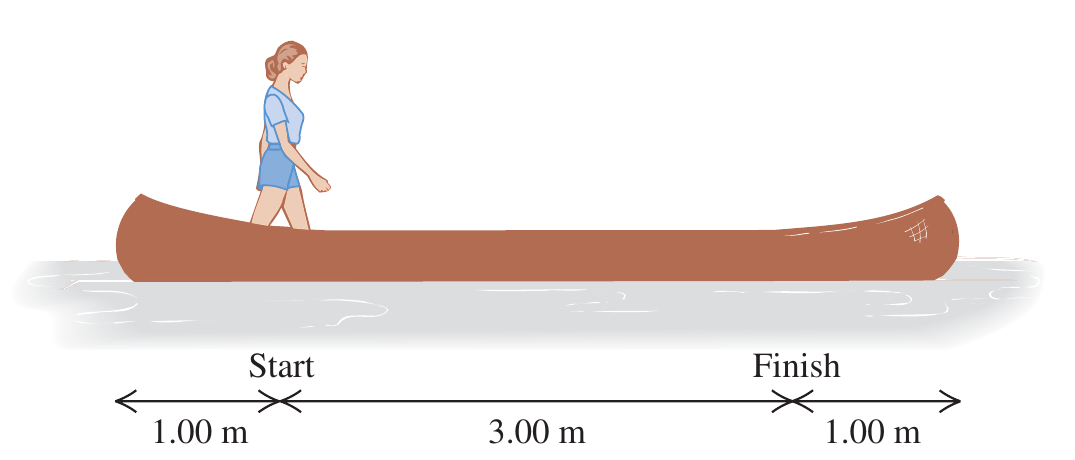
\includegraphics[width=5cm]{canoe.png}
			\vspace{-0.4cm}
		\end{wrapfigure}
		\textbf{[Walking in a boat]} A \SI{45.0}{\kilogram} woman stands up in a \SI{60.0}{\kilogram} canoe of length \SI{5.00}{\meter}. She walks from a point \SI{1.00}{meter} from one end to a point \SI{1.00}{meter} from the other end. If the resistance of the water is negligible, how far does the canoe move during the process?
	\end{shaded}
	
	The first time I attempted this question, I obtained $S_c = \SI{2.25}{\meter}$ via 2 different (but equally incorrect) methods. Should I have checked the sanity of the answer, I would have immediately rejected this answer as incorrect. 
	
	The answer that I have obtained $(S_c = \SI{2.25}{\meter})$ implied that in fact, the woman has only moved $(3.00 - 2.25 = 0.75)$ to the right relative to the stationary river bank. How can it be that the less massive woman undergoes a smaller displacement than the more massive canoe?
	
	Indeed, this does not make sense. Upon further checking, we realize that the answer is not $\SI{2.25}{\meter}$ but $\SI{1.29}{\meter}$.

	
	\section{Dimensional Analysis}
	One of the most powerful problem solving technique is the art of \textbf{\textit{Dimensional Analysis}}. 
	
	The idea behind it is fairly straightforward, that is that all units in an equation must be homogeneous on the left and right hand side. You cannot have a ball that weighs \SI{5}{\meter} or a car that is travelling at \SI{5}{\second}. These simply don`t make sense. 
	
	While they cannot ensure that your answers are right, they can tell you when they are clearly wrong. 
	
	This technique is also a good way to tackle questions in which they want you to choose between several expressions for a certain value: you check if the expression gives the correct dimensions. 
	
	For a more detailed explanation and write up, refer to the attached \textbf{Morins Appendix B}.
	
	\section{Checking Limits}
	A very important part in checking 
	
	For a more detailed explanation and write up, refer to the attached\textbf{ Morins Appendix C}.
	
	TODO: make a table of general order of magnitudes
	\section{ELI5 Method}
	One good way to tackle complicated question is to use the method of reduction. You might be familiar with the concept of ELI5 (Explain like I'm 5 years old). The method of reduction is exactly in the spirit of that:
	
	You try to reduce what you need to find in order to make the problem more approachable, especially if you do not know how to start. 
	
	You can also call this the working backwards method. 
	
	For example, if the question asks for the value of $a$, by reasoning you could say ``If I knew $b$, I would be able to find $a$", and then you go further and realize ``Ah, if I knew $c$, I would be able to find $b$". You keep doing this until you get to something that you know how to find, and you start from there. 
	
	TODO: example question.
	
	\section{When to use vectors and when to not use them}
	With everything in physics seemingly a vector, it might surprise you that sometimes, it is actually easier to solve to solve a question if you disregard the vector aspects of the problem at the start, and just work with the magnitudes of each concerned vector.
	
	In fact, at this point, after doing so many physics questions, you should've already have an intuition about this whole concept.
	
	We shall illustrate this with a few examples: s
\end{document}